\documentclass{beamer}
\mode<presentation>
\usetheme{CambridgeUS}
\usepackage[russian]{babel}
\usepackage[utf8]{inputenc}
\usepackage[T2A]{fontenc}
\usepackage{sansmathaccent}

\usepackage{verbatim}
\usepackage{alltt}

\pdfmapfile{+sansmathaccent.map}
\title[Software Design]{Объекты классов и полиморфизм}
\author{Наумов Д.А., доц. каф. КТ}
\date[14.10.2019] {Основы программной инженерии, 2019}

\begin{document}

%ТИТУЛЬНЫЙ СЛАЙД
\begin{frame}
  \titlepage
\end{frame}
  
%СОДЕРЖАНИЕ ЛЕКЦИИ
\begin{frame}
  \frametitle{Содержание лекции}
  \tableofcontents  
\end{frame}

\section{Статическое и дианмическое связывание типов}
\begin{frame}
\begin{block}{Связывание}
привязка тела функции к месту ее вызова.
\end{block}
\textit{В процедурных языках} задача связывания решается:
\begin{itemize}
\item на этапе компиляции (если определение функции находится в том же модуле, что и обращение к ней);
\item на этапе компоновки (если определение функции находится в другом модуле). 
\end{itemize}
\textit{В объектно-ориентированных языках} переменная-указатель
на объект базового типа может в действительности быть связана с объектом 
производного типа, что делает в общем случае невозможным установление
действительного экземпляра метода, который нужно вызвать, в момент трансляции или компоновки.
\end{frame}

\begin{frame}{Статическое связывание - установление типов во время компиляции}
\begin{figure}[h]
\centering
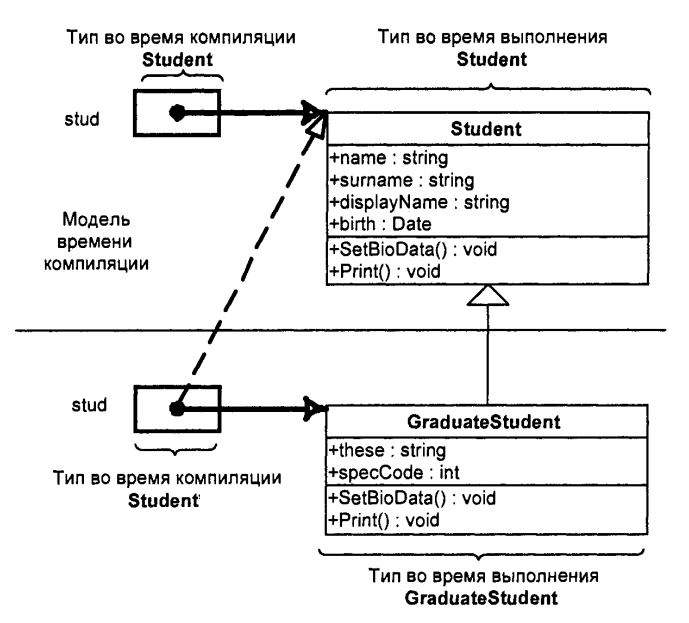
\includegraphics[scale=0.4]{images/lec07-pic01.png}
\end{figure}
\end{frame}

\begin{frame}{Статическое связывание - установление типов во время компиляции}
\begin{figure}[h]
\centering
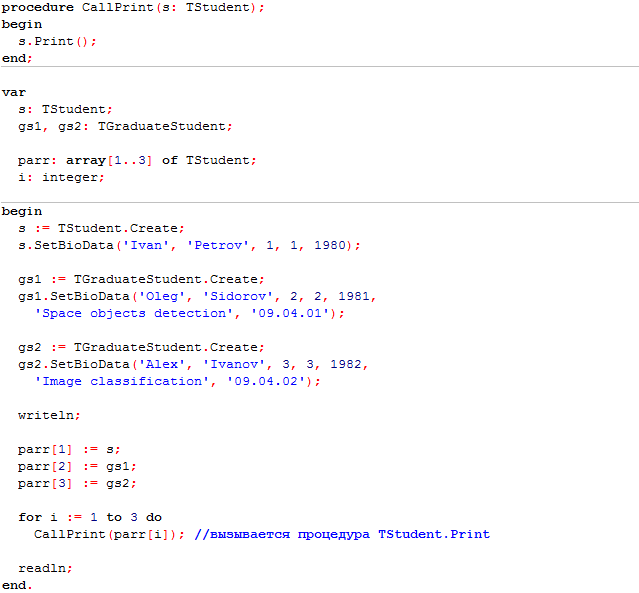
\includegraphics[scale=0.4]{images/lec07-pic02.png}
\end{figure}
\end{frame}

\begin{frame}{Статическое связывание}
\begin{itemize}
\item Во время компиляции невозможно установить, на объект какого типа будет указывать \textit{stud} во время выполнения: на объект типа \textit{student} или на объект производного типа (например, GraduateStudent);
\item Гарантируется, что объект, передаваемый функции CaliPrint() в качестве
аргумента, может быть безопасно и корректно преобразован к типу TStudent
\item Модель времени компиляции в этом случае является моделью времени выполнения. 
\item Даже если в действительности stud связан с объектом типа GraduateStudent, в соответствии с механизмом
статического связывания вызываться всегда будет версия функции Print, объявленная в классе TStudent
\end{itemize}
\end{frame}

\begin{frame}{Статическое связывание}
Можно попытаться <<уговорить>> компилятор, воспользовавшись явным преобразованием типа:
\begin{figure}[h]
\centering
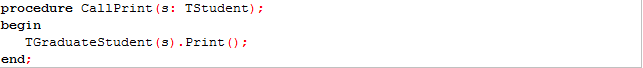
\includegraphics[scale=0.4]{images/lec07-pic03.png}
\end{figure}
Но для переменной типа TStudent результат будет непредсказуем:
\begin{figure}[h]
\centering
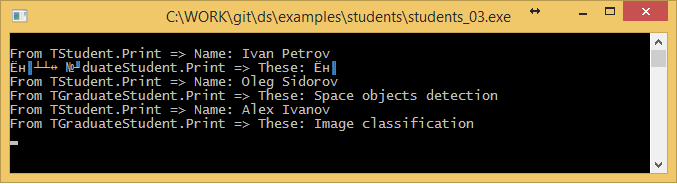
\includegraphics[scale=0.4]{images/lec07-pic04.png}
\end{figure}
\end{frame}

\begin{frame}{Статическое связывание}
Небезопасное преобразование типа:
\begin{figure}[h]
\centering
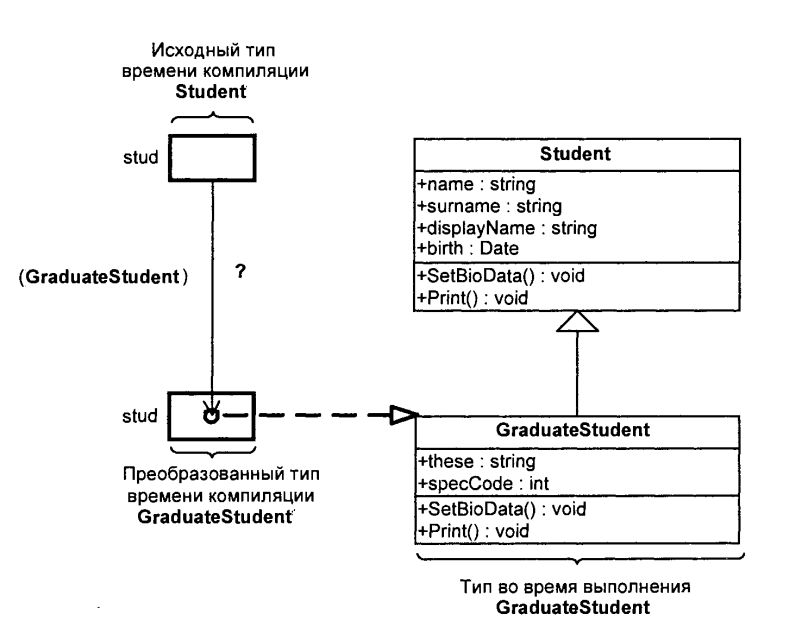
\includegraphics[scale=0.4]{images/lec07-pic05.png}
\end{figure}
\end{frame}

\begin{frame}{Динамическое связывание - установление типов во время выполнения}
\begin{itemize}
\item Механизм реализации динамического связывания основан на использовании виртуальных (перезаписываемых, замещающих) функций.
\item Для того чтобы объявить для некоторого метода необходимость реализовать применительно к этому методу модель позднего связывания, используется ключевое слово virtual. 
\end{itemize}
\begin{figure}[h]
\centering
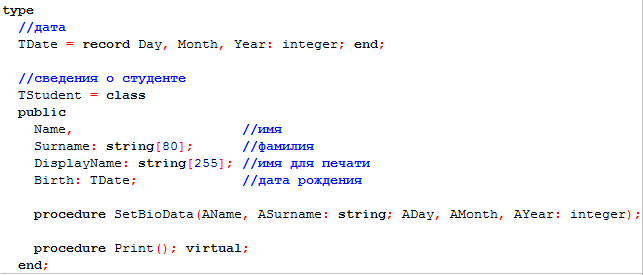
\includegraphics[scale=0.4]{images/lec07-pic06.png}
\end{figure}
\end{frame}

\begin{frame}{Динамическое связывание - установление типов во время выполнения}
\begin{itemize}
\item Для того чтобы метод оставался виртуальным в классе-потомке, используется ключевое слово override. 
\end{itemize}
\begin{figure}[h]
\centering
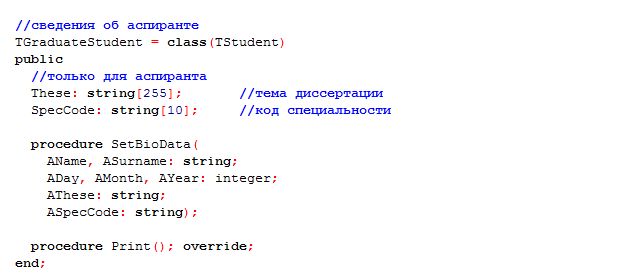
\includegraphics[scale=0.6]{images/lec07-pic07.png}
\end{figure}
\end{frame}

\begin{frame}{Динамическое связывание - установление типов во время выполнения}
\begin{figure}[h]
\centering
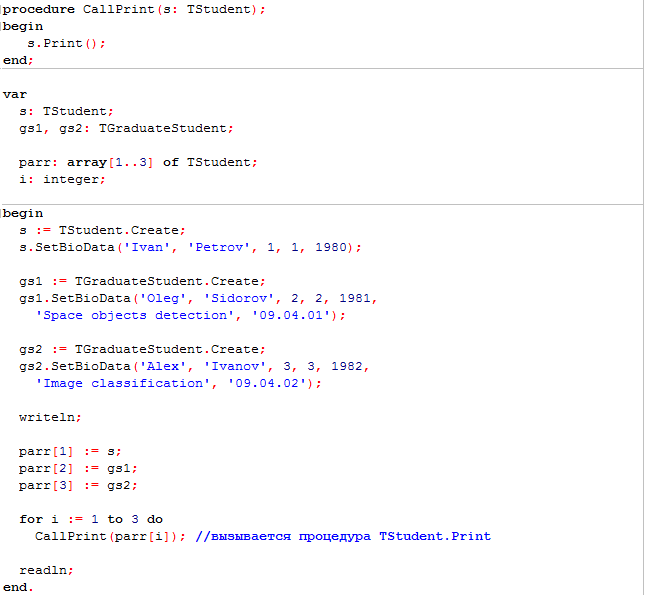
\includegraphics[scale=0.4]{images/lec07-pic08.png}
\end{figure}
\end{frame}

\begin{frame}{Динамическое связывание - установление типов во время выполнения}
\begin{figure}[h]
\centering
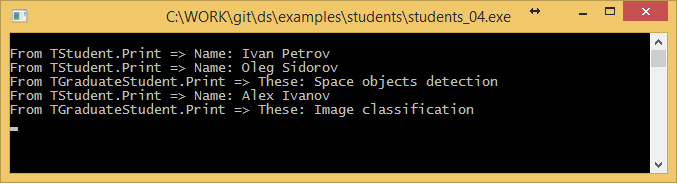
\includegraphics[scale=0.4]{images/lec07-pic09.png}
\end{figure}
\end{frame}

\section{Таблица виртуальных функций}

\begin{frame}{Таблица виртуальных функций}
\begin{itemize}
\item для каждого класса создается специальная таблица, содержащая адреса виртуальных функций, объявленных в этом классе;
\item в определение класса добавляется скрытый член класса — указатель на таблицу виртуальных функций. 
\item адреса одноименных виртуальных функций разных классов, находящихся в отношении наследования, помещаются в ячейки таблицы VTable с одинаковыми индексами.
\item если какая-либо виртуальная функция не перезаписывается в производном классе, в таблицу виртуальных функций помещается адрес соответствующей функции базового класса.
\end{itemize}
\begin{figure}[h]
\centering
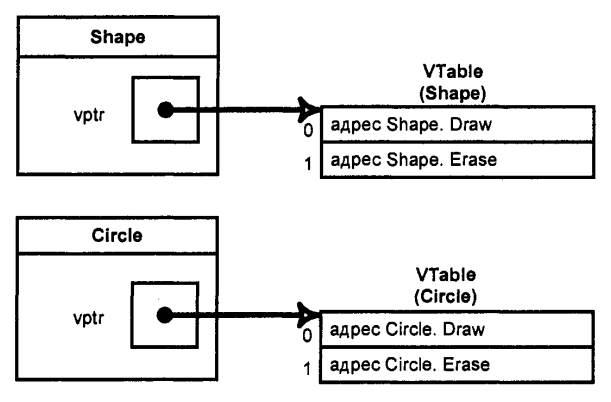
\includegraphics[scale=0.4]{images/lec07-pic10.png}
\end{figure}
\end{frame}

\begin{frame}{Выбор правильной виртуальной функции}
\begin{figure}[h]
\centering
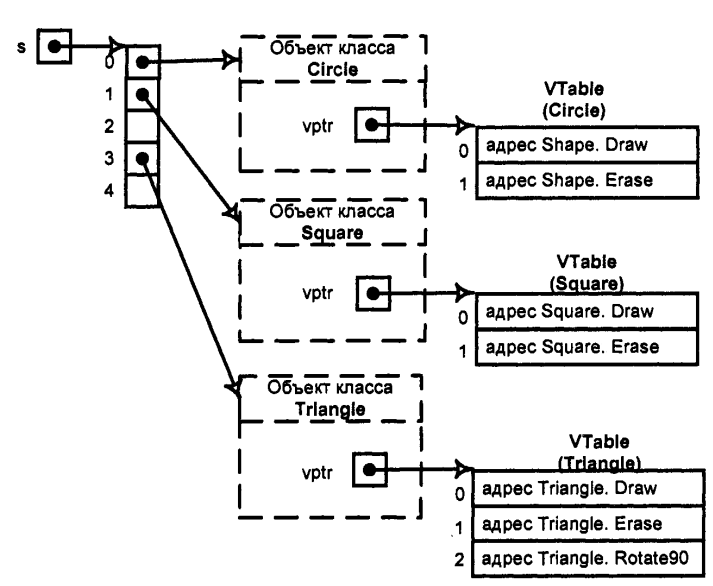
\includegraphics[scale=0.4]{images/lec07-pic11.png}
\end{figure}
\end{frame}

\section{Чисто вирутальные функции и абстрактные классы}

\begin{frame}{Чисто вирутальные функции и абстрактные классы}
\begin{itemize}
\item В ряде случаев уровень абстрагирования, представляемый базовым классом,
не подразумевает какую-либо практическую реализацию некоторых (или всех) методов класса. 
\item В этом случае базовый класс рассматривается как выразитель некоторой абстрактной концепции, предоставляя не реализацию методов, а общий интерфейс, подходящий для работы с элементами такого типа.
\end{itemize}
\begin{figure}[h]
\centering
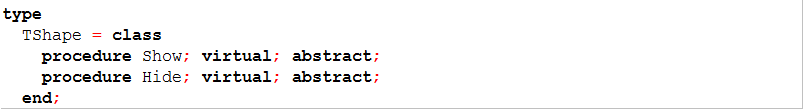
\includegraphics[scale=0.5]{images/lec07-pic12.png}
\end{figure}
\begin{block}{Абстракный класс}
Класс, содержащий хотя бы одну чисто виртуальную функцию.
\end{block}
Объекты абстрактного класса создавать нельзя.
\end{frame}

\section{Приведение типов}

\begin{frame}{Приведение типов}
Использование \textbf{механизма приведения типов} позволяет осуществить преобразование указателя на базовый тип к указателю на производный тип.
\begin{figure}[h]
\centering
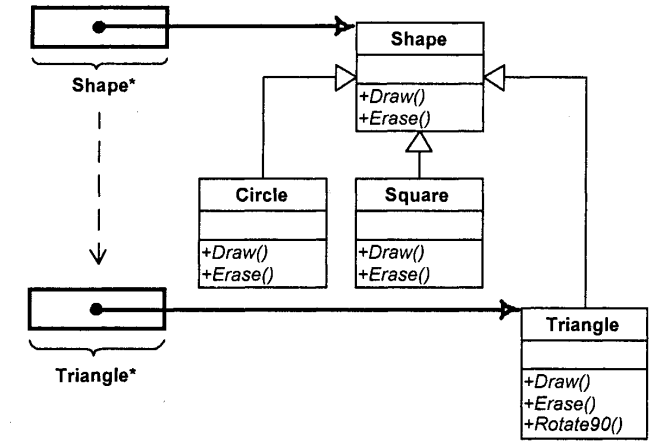
\includegraphics[scale=0.5]{images/lec07-pic13.png}
\end{figure}
В отличие от повышающего преобразования, попытка понижающего преобразования может окончиться неудачей.
\end{frame}

\begin{frame}{Приведение типов}
\begin{figure}[h]
\centering
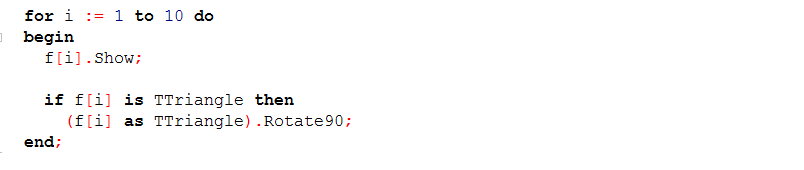
\includegraphics[scale=0.5]{images/lec07-pic14.png}
\end{figure}
В отличие от повышающего преобразования, попытка понижающего преобразования может окончиться неудачей, поэтому требуется проверка.
\begin{figure}[h]
\centering
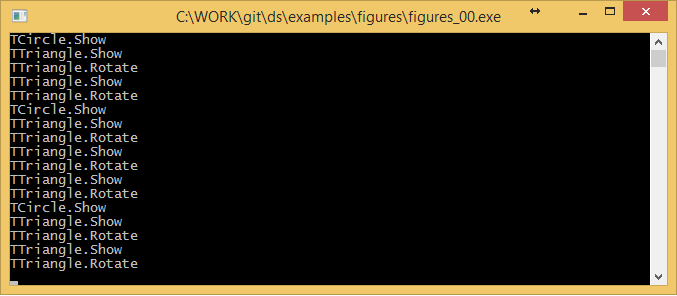
\includegraphics[scale=0.4]{images/lec07-pic15.png}
\end{figure}
\end{frame}

\end{document}
